\lstdefinestyle{mystyle}{
    backgroundcolor=\color{CadetBlue!15!white},   
    commentstyle=\color{Red3},
    numberstyle=\tiny\color{gray},
    stringstyle=\color{Blue3},
    basicstyle=\footnotesize\ttfamily,
    breakatwhitespace=false,         
    breaklines=true,                 
    numbers=left,                    
    numbersep=5pt,                  
    showspaces=false,                
    showstringspaces=false,
    showtabs=false,                  
    tabsize=2,
    language=Python,
    basicstyle=\footnotesize\ttfamily,
	keywordstyle=\color{blue}\footnotesize\ttfamily,
	stringstyle=\color{red}\footnotesize\ttfamily,
    commentstyle=\color{green}\footnotesize\ttfamily,
    morecomment=[l][\color{magenta}]{\#}
}%
\lstset{language=Python,style={mystyle}}%


\chapter{Estado del arte}
\label{estadoDelArte}


Para lograr atributos de calidad en el software, tales como modificabilidad, reusabilidad o mantenibilidad, es fundamental realizar un diseño del mismo basado en estilos arquitectónicos y patrones de diseño \cite{Gamma:1995:DPE:186897,ShawGarlan1996,buschmann,ghezzi2003,DBLP:books/daglib/0030743,bass2003}. Es decir, aplicar las nociones centrales de la \glsentrylong{IS} (\gls{IS}).

Los sistemas de software para robots por lo general poseen alguna de las siguientes características: son distribuidos, embebidos, en tiempo real o manejan muchos datos \cite{noergaard2005embedded, braunl2003embedded}. Su complejidad no termina ahí, deben encargarse del acceso al hardware, los algoritmos de navegación y decisión, entre otras responsabilidades, por lo tanto, muchas veces el diseño es considerado menos prioritario por quienes desarrollan este tipo de sistemas. Esto provoca que el esfuerzo se concentre en solucionar inconvenientes de implementación y no en diseñar cumpliendo los principios de la \gls{IS} \cite{Brugali2009}.

En los trabajos que incluyen información relacionada con el diseño del software \cite{bad-desing-auto,bad-desing-implantable,code-1,code-2,Zhang2009,bad-design-uml,bad-design-robot}, se observa que esta suele ser escasa y, en general, representada mediante diagramas de flujo. Por ejemplo, en la Figura \ref{flujo} puede verse cómo se presenta el diseño del sistema principal de control de dirección asistida de un vehículo. Este se muestra mediante un diagrama de flujo con el propósito de ilustrar el comportamiento del software, lo cual evidencia que la implementación se ha realizado siguiendo un criterio de división funcional del código. Por otro lado, en diversos trabajos se identifican prácticas de programación poco adecuadas, tales como el uso excesivo de estructuras condicionales anidadas (\textit{ifs}) y la escasa utilización de funciones, lo que revela una deficiente modularidad. Un ejemplo de ello se presenta en el Código \ref{ifanidados}, donde se observan hasta tres niveles de anidamiento. Este tipo de enfoque y el uso de prácticas no recomendables resultan en un código menos modificable, reutilizable y mantenible \cite{Parnas1972}.

\begin{figure}[H]
	\centering
	\caption{Diagrama de flujo que describe el comportamiento del programa principal de control en \cite{bad-desing-auto}}.
	\label{flujo}
    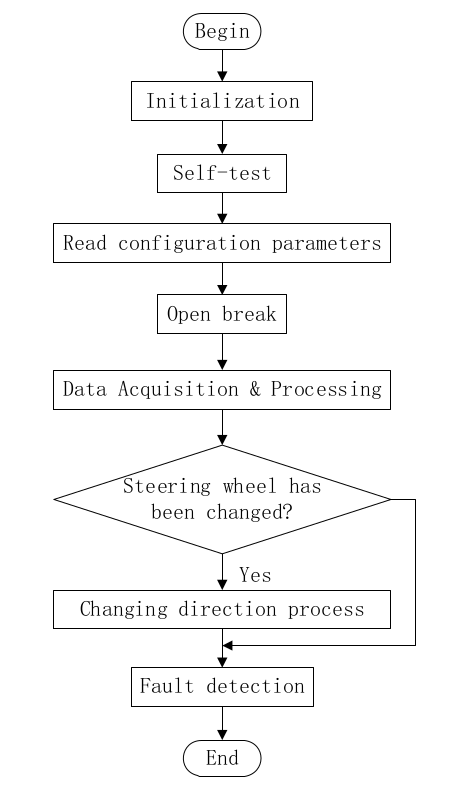
\includegraphics[width=0.5\linewidth]{main_flujo.png}
\end{figure}

\begin{lstlisting}[caption=Extracto de código de \cite{code-2}.,label={ifanidados}]
 if _py_timestamp is not None:
        # Initialize from PyTimestamp, if available.
        self._py_timestamp = _py_timestamp
    elif timestamp is not None:
        # If Timestamp is available, copy its contents.
        self._py_timestamp = timestamp._py_timestamp
    else:
        if is_top and not is_bottom and coordinates is None:
            self._py_timestamp = PyTimestamp(coordinates, is_top, is_bottom)
        elif is_bottom and not is_top and coordinates is None:
            self._py_timestamp = PyTimestamp(coordinates, is_top, is_bottom)
        elif coordinates is not None and not is_bottom and not is_top:
            self._py_timestamp = PyTimestamp(coordinates, is_top, is_bottom)
        else:
            raise ValueError(
                "Timestamp should either have coordinates"
                "or be either Top or Bottom"
             )
\end{lstlisting}


En contraposición a estos trabajos, existen otros \cite{good-desing-agrobot,good-desing-street} que tienen en cuenta algunos principios fundamentales de la \gls{IS} a la hora de diseñar y destinan esfuerzo en crear software de cierta calidad. Sin embargo, no se evidencia la aplicación de patrones de diseño.

Por otro lado, existen múltiples trabajos que abordan supuestos patrones de diseño aplicados a ámbitos particulares, inspirándose en la manera de documentar que utilizan los autores en \cite{Gamma:1995:DPE:186897}. Sin embargo, como veremos, no cumplen con los criterios establecidos para ser considerados patrones de diseño.

Entre ellos encontramos los siguientes:

\begin{itemize}
\item \cite{enjambre}, se definen patrones de diseño para \gls{enjambresroboticos} en conjunto a un formato de documentación particular. Los patrones se centran en diferentes comportamientos comunes que deben realizar los robots en este tipo de sistemas, como intercambiar información o llevar a cabo ciertas interacciones.

\item \cite{patterns_2013}, presenta tres patrones orientados al control autónomo de robots. Parecen estar más cerca de arquitecturas, ya que definen el funcionamiento general de ciertos sistemas sin definir módulos y sus interfaces.

\item \cite{stable} donde se describen patrones que ayudan a desarrollar familias de sistemas robóticos estables, definiendo familia de sistemas como ``estable'' a una familia de sistemas modelada, diseñada e implementada de manera que las aplicaciones específicas de dicha familia puedan desarrollarse reutilizando, adaptando y especializando conocimientos, arquitecturas y componentes existentes.

\item \cite{critical} se encuentran patrones de diseño tanto para hardware como software aplicados a sistemas donde la seguridad es crítica debido a su naturaleza. Las aplicaciones de este tipo pueden provocar consecuencias considerables en caso de fallos. La mayoría de los supuestos patrones de diseño descriptos se centran en la redundancia y control de resultados. Además de documentarlos, el autor agrega un análisis de impacto en el coste computacional, con el fin de justificar que su aplicación no genera un impacto significativo.

\end{itemize}

Podría pensarse entonces que existen múltiples trabajos que abordan patrones de diseño para sistemas embebidos de control o robóticos, sin embargo, no es exactamente así. En los trabajos mencionados, se utiliza el concepto de patrón de diseño, pero no al nivel de diseño que se trabaja en la IS. Los patrones presentados son \textit{soluciones probadas para ciertos problemas recurrentes}, pero el cambio \textbf{no} aparece involucrado entre esos problemas. Es decir, los autores detallan cómo aplicar una solución a diversos inconvenientes comunes en sus áreas de estudio, pero no incluyen al diseño para el cambio a la hora de su confección. Por ejemplo, un patrón de diseño presentado en \cite{robotArg} es \textit{Patrón de Diseño para el control de un robot diferencial}. Este provee una solución que permite implementar de manera simple un sistema de control específico. Pero no se pone al diseño para el cambio como una variable a tener en cuenta, la solución no lo considera. Por lo que el resultado de su aplicación no es software preparado para el cambio.

En algunos de los trabajos previamente enumerados, y como veremos más adelante en la tesina en el libro de \cite{douglass}, lo que allí se denominan patrones de diseño en realidad corresponden a patrones idiomáticos. Estos también conocidos como \textit{idioms}, son soluciones recurrentes a problemas específicos de implementación que aprovechan las características particulares de un lenguaje de programación. Estos patrones encapsulan prácticas efectivas y convenciones que han demostrado ser útiles para resolver ciertos desafíos técnicos de forma eficiente y elegante dentro del contexto de un lenguaje concreto. A diferencia de otros enfoques más abstractos, los \textit{idioms} operan a nivel del código, abordando aspectos como el manejo de memoria, el control de errores, la gestión de recursos o el uso avanzado de estructuras del lenguaje. Su valor radica en facilitar la implementación de soluciones, al mismo tiempo que aprovechan al máximo las capacidades del compilador o del entorno de ejecución. Debido a su naturaleza dependiente del lenguaje, un \textit{idiom} que es válido y útil en un lenguaje puede no tener sentido o incluso ser contraproducente en otro \cite{buschmann1996posa1}.

Además, en estos trabajos no se estudian módulos ni interfaces, sino componentes del sistema, algo más parecido a una arquitectura de software. De hecho, se llegan a documentar patrones de diseño para hardware\footnote{Un patrón de diseño para hardware es una solución reutilizable y probada a un problema recurrente en el diseño de sistemas físicos o digitales. Suele describir estructuras o componentes de hardware que pueden ser replicados o adaptados, facilitando la estandarización, la reutilización y la eficiencia en el desarrollo.}, como ocurre con muchos de los patrones definidos en \cite{critical}. En el trabajo \cite{stable} se considera el hecho de reutilizar software, pero los patrones descriptos corresponden a un nivel de abstracción superior al que se busca en esta tesina. Tratan la interacción de diferentes componentes, similar a una arquitectura de software.

De todas formas, es notable como la comunidad de Robótica ha comenzado a discutir sobre la necesidad de aplicar técnicas y principios de IS para construir software robótico mantenible, reusable y modificable \cite{Brugali2009, mejoras-2}. Una prueba del interés son desarrollos como \cite{FernandezMadrigal2003, model,model1,model2,model3}, en los cuales se integran de diferentes maneras, prácticas de la \gls{IS} en el desarrollo de sistemas embebidos. Por un lado, desarrollando \glspl{framework} y arquitecturas orientadas a este tipo de software, como también definiendo metodologías de trabajo. Estos \glspl{framework} no son los únicos orientados a este tipo de sistemas, existen por ejemplo \cite{framework-1, framework-ros}, los cuales son una combinación de sistema operativo y \textit{framework}. Representan fuertes herramientas para el desarrollo, principalmente, solucionan algunos inconvenientes recurrentes y le quitan responsabilidades al desarrollador resolviendo cuestiones relacionadas con el acceso al hardware, concurrencia, etc.. Es decir, proveen una capa de abstracción a partir de la cual los desarrolladores pueden empezar a trabajar. Son ampliamente utilizados en la industria y aplicados a grandes sistemas. No así para aplicaciones de menor tamaño, ya que proveen una estructura mayor a la necesaria, complejizando innecesariamente el sistema.

Otra prueba de interés son trabajos como \cite{Shin15fase}, en los cuales se propone incorporar formación relacionada con la \gls{IS} en cursos de robótica y sistemas embebidos, otorgando igual énfasis tanto a la \gls{IS} como a la Robótica. El objetivo del curso es enseñar a los estudiantes cómo aplicar los principios de la \gls{IS} al campo de la Robótica. En particular, se dan dos lecturas principales que contienen los conceptos de patrones de diseño y arquitectura de software. En la primera lectura se trabaja sobre los patrones \textit{Observer}, \textit{State}, \textit{Strategy} y \textit{Visitor}. El patrón \textit{Observer} se utiliza extensivamente en \gls{ros}\cite{framework-ros} para la comunicación. El patrón \textit{State} es útil para implementar el algoritmo de evitación de obstáculos, que consta de varios estados. El patrón \textit{Strategy} permite intercambiar fácilmente diferentes estrategias de planificación de rutas. El patrón \textit{Visitor} es útil para implementar diferentes métodos de predicción y actualización en la localización. En la segunda lectura, se discuten diferencias entre múltiples arquitecturas utilizadas en el campo, tales como CARMEN \cite{carmen}, MOOS \cite{moos}, Microsoft Robotics Studio \cite{microsoft} y \gls{ros}\cite{framework-ros}. 

Una de las principales motivaciones es la introducción de la robótica al mercado de consumo masivo fomentando la demanda de reducir los costos del software preservando sus cualidades \cite{Brugali2009}. A medida que los sistemas embebidos incluyen más funciones para nuevos servicios, el software crece gradualmente en tamaño, y los costos y el tiempo de desarrollo también \cite{model2}. En particular, el diseño orientado al cambio, es una de las herramientas claves de la \gls{IS} para conseguirlo, ya que promueve la reusabilidad del software, haciéndolo aplicable a distintos proyectos y entornos. Esta es una muestra de que la implementación de patrones de diseño es una solución potencialmente útil y deseada.

En línea con este enfoque, en esta tesina se presentarán algunos problemas recurrentes en el dominio de la robótica y se propondrán algunas soluciones de diseño basadas en patrones de diseño con el objetivo de construir software de calidad.

